\begin{frame}
\frametitle{Dockefile}

A docker can be created by hand

\begin{itemize}
\item pull an image
\item star a container
\item modify the container
\item commit the changes 
\end{itemize}

this is more or less the process for creating a reusable container \textit{an Image}
\end{frame}

\begin{frame}
\frametitle{Dockerfile}

By \textit{hand} is good for practicing or testing but is very bad for 
\begin{itemize}
\item reproducibility
\item automation
\item dependencies
\end{itemize}
\end{frame}

\begin{frame}
\frametitle{Dockerfile}

By \textit{hand} is good for practicing or testing but is very bad for 

\begin{itemize}
\item \textit{reproducibility}: lost the history of the commands that create the final image
\item automation
\item dependencies
\end{itemize}
\end{frame}

\begin{frame}
\frametitle{Dockerfile}

By \textit{hand} is good for practicing or testing but is very bad for 

\begin{itemize}
\item reproducibility
\item \textit{automation}: images are lost because some disaster and eveything was on a local machine
\item dependencies
\end{itemize}
\end{frame}

\begin{frame}
\frametitle{Dockerfile}

By \textit{hand} is good for practicing or testing but is very bad for 

\begin{itemize}
\item reproducibility
\item automation
\item \textit{dependencies}: images are build from other images and something must be changed in the original image
\end{itemize}
\end{frame}

\begin{frame}
\frametitle{Dockerfile}
\framesubtitle{what is it?}

A simple text files with all the instructions for

\begin{itemize}
\item start (PULL) from a (public) Linux distribution
\item install software
\item configure the installation
\item configure the container for running automatically
\end{itemize}
\end{frame}

\begin{frame}[fragile]
\frametitle{Dockerfile}
\framesubtitle{what is it?}

The most minimal \lstinline!Dockerfile!
\begin{lstlisting}
FROM ubuntu:18.04
\end{lstlisting}

\textit{Note} by convention \lstinline!Dockerfile! is the name to use for the file containing the instructions.
\end{frame}


\begin{frame}[fragile]
\frametitle{Dockerfile}
\framesubtitle{How to use it}

A \lstinline!Dockerfile! can be used for building a new image

\begin{lstlisting}
 $ docker build -t origin .
 Sending build context to Docker daemon  2.048kB
 Step 1/1 : FROM ubuntu:18.04
  ---> cd6d8154f1e1
  Successfully built cd6d8154f1e1
  Successfully tagged origin:latest
\end{lstlisting}

A new image is created with the \lstinline!sha256! \lstinline!cd6d8154f1e1! called \lstinline!origin! and the version, in this case by default \lstinline!Docker! assign the tag \lstinline!latest!
\end{frame}

\begin{frame}[fragile]
\frametitle{Dockerfile}
\framesubtitle{FROM}

Start from a Linux distribution or previous installations/images

\begin{lstlisting}
FROM <image> [AS <name>]

FROM <image>[:<tag>] [AS <name>]

FROM <image>[@<digest>] [AS <name>]
\end{lstlisting}
\end{frame}

\begin{frame}[fragile]
\frametitle{Dockerfile}
\framesubtitle{LABEL}

Metadata are useful in order to describe the image, making it more consumable by others

\lstinline!LABEL <key>=<value> <key>=<value> <key>=<value> ...!

\begin{lstlisting}
LABEL org.ingm.group="Your Boss name"
LABEL maintainer="Bonnal Raoul J.P. <bonnal@ingm.org>"
LABEL project="Elixir Test"
LABEL description="Dockerfile example \
with multiple lines."
LABEL version="1.2"
 
LABEL maintainer=''bonnal@ingm.org''
\end{lstlisting}

User is free to use any kind of \lstinline!key=val! convention but the \textit{reverse DNS} notation.
\end{frame}

\begin{frame}[fragile]
\frametitle{Dockerfile}
\framesubtitle{ENV}

Environment variables can be set inside the container

\begin{lstlisting}
ENV <key> <value>
ENV <key>=<value> ...
\end{lstlisting}

\begin{lstlisting}
ENV software="samtools" description=A\ great\ piece\ of\ software
    author=someone
\end{lstlisting}	
and
	
\begin{lstlisting}
ENV software samtools
ENV description A great piece of software
ENV author someone
\end{lstlisting}

these variable are available during the building process and when the container is running
\end{frame}

\begin{frame}[fragile]
\frametitle{Dockerfile}
\framesubtitle{WORKDIR}

Sets the working directory for the following \textit{instructions}

\begin{lstlisting}
ENV MYSUBDIR mytmp
RUN mkdir /opt/$MYSUBDIR
WORKDIR /opt/$MYSUBDIR
RUN pwd
\end{lstlisting}

Works for \lstinline!RUN!, \lstinline!CMD!, \lstinline!ENTRYPOINT!, \lstinline!COPY! and \lstinline!ADD!
\end{frame}

\begin{frame}[fragile]
\frametitle{Dockerfile}
\framesubtitle{injecting files}

To fully customize the image, external files can be included. To achieve this \textit{Docker} provides two different tools

\begin{itemize}
\item \lstinline!ADD!
\item \lstinline!COPY!
\end{itemize}
\end{frame}

\begin{frame}[fragile]
\frametitle{Dockerfile}
\framesubtitle{ADD}

\begin{lstlisting}
ADD [--chown=<user>:<group>] <src>... <dest>
ADD [--chown=<user>:<group>] ["<src>",... "<dest>"]
\end{lstlisting}
\begin{itemize}
\item Digest URLs, download
\item Unpack archives (identity, gzip, bzip2 or xz)
\item Does not perform authentication
\item At every build it is re excuted
\end{itemize}
\end{frame}

\begin{frame}[fragile]
\frametitle{Dockerfile}
\framesubtitle{COPY}

\begin{lstlisting}
COPY [--chown=<user>:<group>] <src>... <dest>
COPY [--chown=<user>:<group>] ["<src>",... "<dest>"]
\end{lstlisting}

\begin{itemize}
\item Relative path outside of context does not work
\item Works only with local files or directory
\item Can copy files from source location to a previous build stage \lstinline!FROM!
\item NO URLs
\item NO auto unpacking
\end{itemize}
\end{frame}

\begin{frame}[fragile]
\frametitle{Dockerfile}
\framesubtitle{SHELL}

When commands must be run with a different shell

\begin{lstlisting}
SHELL ["executable", "parameters"]
\end{lstlisting}
\end{frame}

\begin{frame}[fragile]
\frametitle{Dockerfile}
\framesubtitle{USER}

Set the USER to use during when the containers run.
It also set the user for \lstinline!RUN!, \lstinline!CMD!, \lstinline!ENTRYPOINT! following the declaration of \lstinline!USER!

\begin{lstlisting}
USER <user>[:<group>]
USER <UID>[:<GID>]
\end{lstlisting}
\end{frame}

\begin{frame}[fragile]
\frametitle{Dockerfile}
\framesubtitle{RUN}

To customise the installation the user must execute commands.

The commands are run inside a default shell \lstinline!/bin/sh -c!

Use the \lstinline!SHELL! clause to change the shell for the following \lstinline!Dockerfile!

When a \lstinline!RUN! succeed Docker will write a layer.
\end{frame}

\begin{frame}[fragile]
\frametitle{Dockerfile}
\framesubtitle{RUN}

\lstinline!RUN! have two forms:

\begin{lstlisting}
RUN apt-get update
\end{lstlisting}

or use a more explicit form where parameters are passed in a sort of \lstinline!JSON! notation

\begin{lstlisting}
RUN ["apt-get", "update"]
\end{lstlisting}

The JSON form does not create a shell for the command, so variable can not be substituted. To use the shell substitution call the shell first.
\end{frame}

\begin{frame}[fragile]
\frametitle{Dockerfile}
\framesubtitle{RUN}

\begin{lstlisting}
RUN apt-get install -y wget git python3.6
\end{lstlisting}

A \lstinline!RUN! command can span multiple lines


\begin{lstlisting}
RUN apt-get install -y wget \
                       git \
					   python3.6
\end{lstlisting}
\end{frame}

\begin{frame}[fragile]
\frametitle{Dockerfile}
\framesubtitle{RUN}

A \lstinline!RUN! command can be made by multiple commands

\begin{lstlisting}
RUN comamnd1 && command2
\end{lstlisting}

The \lstinline!RUN! will pass and create a layer only if it succeed. Otherwise, Docker will report the original error.
\end{frame}

\begin{frame}[fragile]
\frametitle{Dockerfile}
\framesubtitle{RUN}

Combining commands and spanning the commands on multiple lines helps in readability and building complex configurations.

\begin{lstlisting}
RUN apt-get update &&\
    apt-get install -y wget 
\end{lstlisting}
\end{frame}

\begin{frame}[fragile]
\frametitle{Dockerfile}
\framesubtitle{RUN}

Combining commands and spanning the commands on multiple lines helps in readability and building complex configurations.

\begin{lstlisting}
RUN apt-get update &&\
    apt-get install -y wget \
	                   git \
					   python3.6
\end{lstlisting}
\end{frame}

\begin{frame}[fragile]
\frametitle{Dockerfile}
\framesubtitle{ENTRYPOINT}
Defines a container that runs as an executable

Forms:

\begin{itemize}
\item \textit{exec}: preferred \lstinline!ENTRYPOINT ["executable", "param1", "param2"]!

\item \textit{shell}:  \lstinline!ENTRYPOINT command param1 param2!
\end{itemize}
\end{frame}


\begin{frame}[fragile]
\frametitle{Dockerfile}
\framesubtitle{CMD}
Defines the default behavior for the container.

Forms:
\begin{itemize}
\item \textit{exec}: preferred \lstinline!CMD ["executable","param1","param2"]!
\item default parameters to \lstinline!ENTRYPOINT!: \lstinline!CMD ["param1","param2"]!
\item \textit{shell}: \lstinline!CMD command param1 param2!
\end{itemize}
\end{frame}

\begin{frame}[fragile]
\frametitle{Dockerfile}
\framesubtitle{VOLUME}
It is possible to embed the volume definition at build time.

Any change, at build time, after the definition will be discarded.

\begin{lstlisting}
VOLUME ["/path","..."]

VOLUME /path_a /path_b
\end{lstlisting}

Volumes are:
\begin{itemize}
\item created automatically at run time
\item can be shared between containers with \lstinline!--volumes-from!
\item are anonymous at runtime
\item can be inspected looking at \lstinline!/var/lib/docker/volumes!
\end{itemize}
\end{frame}

\begin{frame}[fragile]
\frametitle{Dockerfile}
\framesubtitle{VOLUME}

Example of creating a \lstinline!VOLUME!

\begin{lstlisting}
FROM ubuntu:18.04
RUN mkdir /opt/elixir-volume
RUN echo "This is a file with a foo text" > /opt/elixir-volume/README.txt
VOLUME ["/opt/elixir-volume"]
\end{lstlisting}
\end{frame}

\begin{frame}[fragile]
\frametitle{Dockerfile}
\framesubtitle{context}

Context defines what is visible at the build time by Docker.
Data inside the \textit{context} are copied in a temporary place where the building process is working. The building process can see only data in that temporary place. 

This process of \textit{building the context} can take a lot of time if files are big and many.

Avoid:
\begin{itemize}
\item huge files
\item temporary or working file
\item backup 
\end{itemize}

in the context.

A lean \textit{context} means quick build.
\end{frame}

\begin{frame}
\frametitle{Dockerfile}
\framesubtitle{validation}

A \textit{Dockerfile} is a text file and Docker keep tracks of changes in the file.

Most of the \textit{instructions} generate a layer. 

Changes to the text are invalidaing all the following \textit{instructions} and they will be re-executed.
\end{frame}

\begin{frame}[fragile]
\frametitle{Dockerfile}
\framesubtitle{example}

\begin{lstlisting}
FROM ubuntu:18.04

LABEL org.ingm.group="Your Boss name"
LABEL maintainer="Bonnal Raoul J.P. <bonnal@ingm.org>"
LABEL project="Elixir Test"
LABEL description="Dockerfile example"
LABEL version="1.2"

RUN apt-get update &&\
    apt-get install -y wget \
	                   git \
					   python3.6
\end{lstlisting}
\end{frame}

\begin{frame}[fragile]
\frametitle{Dockerfile}
\framesubtitle{bulding}

\begin{lstlisting}
$ docker build -t origin .

$ docker build -t origin Dockerfile .

$ docker build -t origin -f /absolute/path/Dockerfile .
\end{lstlisting}
\end{frame}

\begin{frame}
\frametitle{Dockerfile}
\framesubtitle{building}

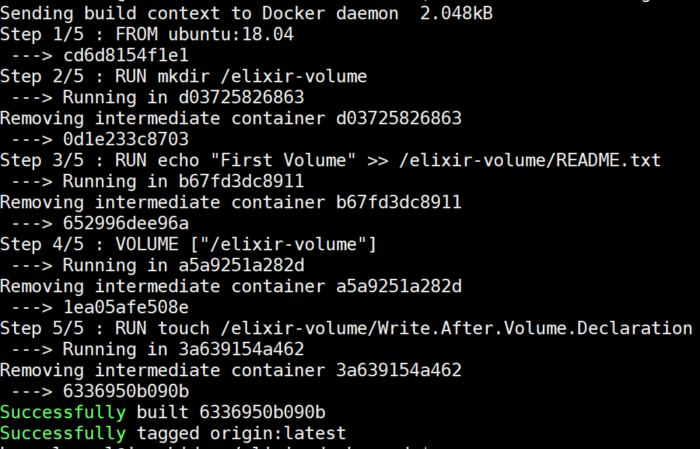
\includegraphics[width=0.8\columnwidth]{./Figure/BuildingDockerfile}
\end{frame}

